\documentclass[pflichtenheft.tex]{subfiles}

\begin{document}

%-------------- PRODUKTEINSATZ ---------------------
\chapter{Produkteinsatz}
Das Produkt dient zur Speicherung und Distribution von Daten mehrerer verteilter Sensoren eines Autos. Dies beinhaltet Informationen wie die Geschwindigkeit, Motortemperatur, Raddrehzahl und ähnliches. Damit bietet es die Möglichkeit, diese Daten  auf einem Smartphone, Laptop oder anderem Computer mit Bildschirm anzuzeigen.


\section{Anwendungsbereiche}
\begin{itemize}
\item
Dieses Produkt dient zum Speichern und Anzeigen von in einem PKW verfügbaren Sensordaten.
\end{itemize}


\section{Zielgruppen}
\begin{itemize}
\item
Private Autofahrer mit oder ohne tieferen technischen Kenntnissen von PKWs. 
\end{itemize}


\section{Betriebsbedingungen}
\begin{itemize}
\item
Der PKW muss über einen OBD2-Anschluss verfügen.
\item
Das Produkt muss Strom aus dem Auto beziehen können.
\item
Für Remote-Zugriff muss eine Netzwerkverbindung vorhanden sein.
\end{itemize}


%--------------- Produktumgebung -------------
\chapter{Produktumgebung}
Das Rahmenwerk und die Module werden in TypeScript\footnote{http://www.typescriptlang.org} programmiert. Der Server wird in node.js\footnote{https://nodejs.org/} laufen. Als Datenbanksystem wird LevelUp\footnote{https://github.com/Level/levelup} verwendet.

\begin{itemize}

\item
Eine Client-Server-Architektur nach dem Thin-Client-Konzept
\item
Auf dem Server läuft der Teil der Software, der die Sensordaten empfängt, einpflegt und über WebRTC an die Endgeräte versendet.
\item
Auf der Clientseite laufen verschiedene Applikationen neben VINJAB. Diese Anwendungen sollen die Software aber nicht beeinflussen und auch nicht von ihr beeinflusst werden.
\end{itemize}

%%%%Fragen
\section*{Testumgebung}
\begin{itemize}
\item
Testfahrzeug: Opel Astra H 1.6 Baujahr 2005
\item
Testfahrzeug: ITK-Engineering Modellauto \\
Ein Modellauto der Firma ITK-Engineering AG, angetrieben über einen Elektromotor. Alle Daten, die hier verfügbar sind, liegen über CAN an.
\item
Raspberry Pi 2 Model B
\item
ASUS BT400 Bluetooth USB Adapter
\item
UMTS-Stick
\item
OBD2-Bluetooth-Adapter ELM327
\end{itemize}


\section{Software}
\begin{itemize}
\item
\textbf{Serverseite:}\\
Ein Debian-Linux-basierter Server, auf dem eine LevelDB-Datenbank läuft.
\item
\textbf{Clientseite:}\\
Web-Browser:
\begin{itemize}
\item
Google Chrome Version 46
\item
Safari Version 9
\item
Firefox Version 42
\item
Google Chrome Android Version 14.10
\end{itemize}
\end{itemize}


\section{Hardware}
\begin{itemize}
\item
\textbf{Serverseite:}\\
Kleincomputer mit:
\begin{itemize}
\item
Broadcom BCM2836 Arm7 Quad Core Processor (900MHz)
\item
1GB RAM
\item
4 x USB 2 ports
\item
Bluetooth-Funktionalität
\end{itemize}
Can-Modul
\item
\textbf{Clientseite:}\\
Standardrechner (min. 1 GHz und 2 GB RAM)\\
Android Smartphone (min. 1 GHz und 1 GB RAM)
\end{itemize}


\newpage
\section{Systemarchitektur}

Das System ist modular aufgebaut. Es gibt pro System genau einen Server. Endgeräte können eine Netzwerkverbindung mit dem Server herstellen. Dabei kann die Verbindung entweder direkt via Wi-Fi im Auto oder entfernt (~\ref{remote}) über das Internet hergestellt werden. (~\ref{firstcon}, ~\ref{connection}) Das soll in der Funktionalität keinen Unterschied machen. Diese Verbindung beruht auf WebRTC\footnote{http://www.webrtc.org} und soll den Datenkanal dieses Protokolls verwenden, um Sensordaten zu übertragen. Des Weiteren ist eine Rückfahrkamera per USB mit dem Server verbunden. Die Kamerabilder werden über den Media Kanal (WebRTC) auf das Endgerät übertragen. Das mit dem Lenkrad markierte Endgerät stellt das Gerät des Fahrers dar. Personenbezogene Daten werden nach Fahrer gespeichert. (~\ref{driver1}, ~\ref{driver2})

\begin{figure}[H]
  	\begin{center}
 		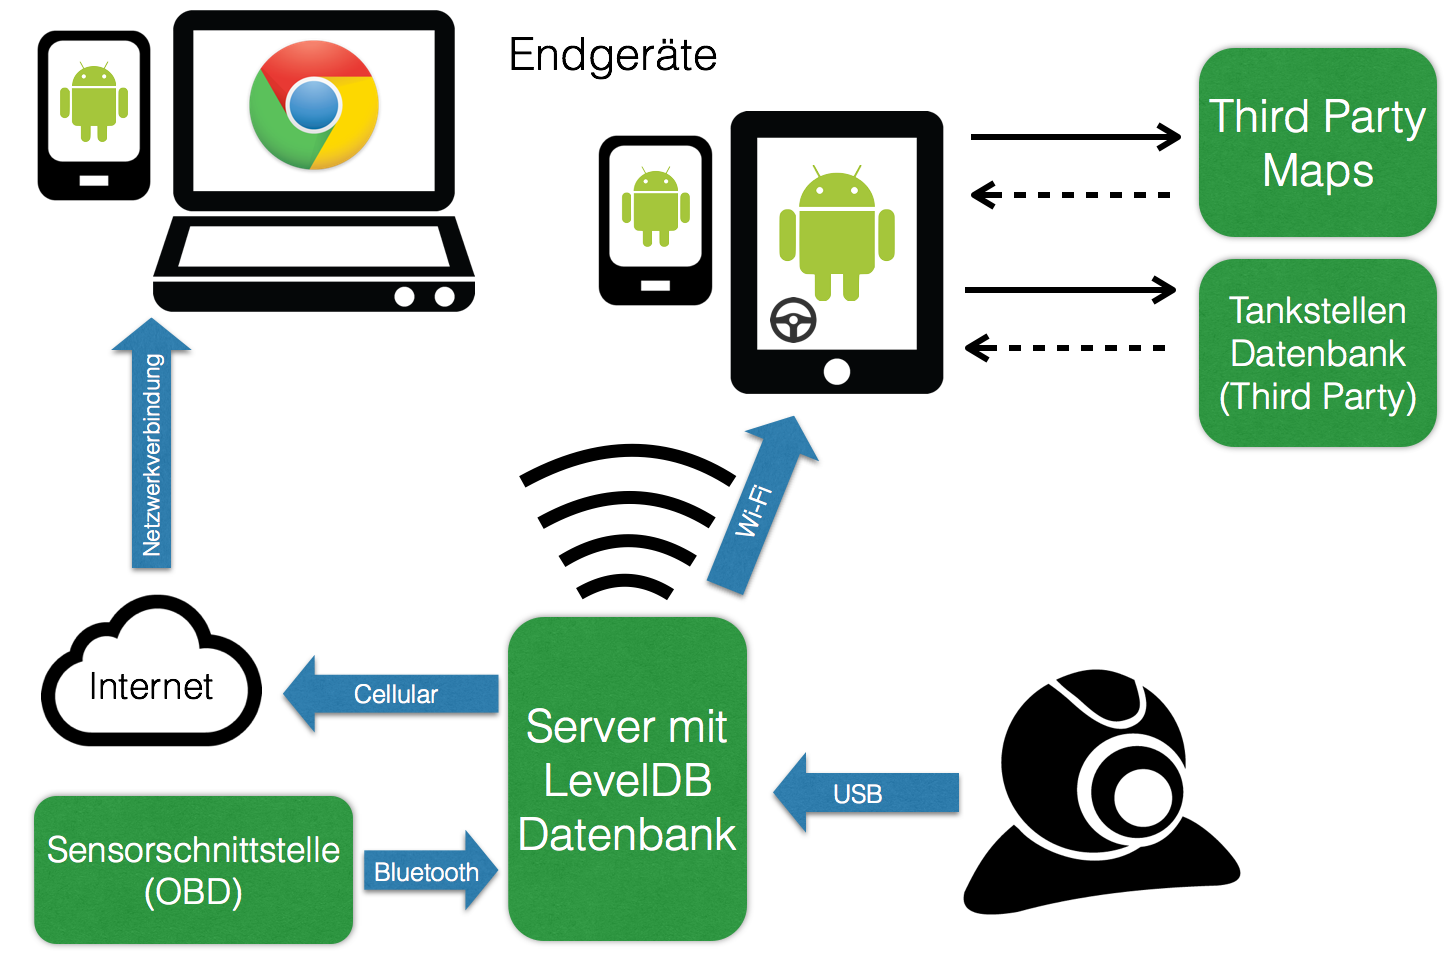
\includegraphics[width=\textwidth]{Images/sysarch.png}
  		\caption{Blockbild der Systemarchitektur}
  	\end{center}
\end{figure}

\end{document}



